\chapter{Web Portal Design}
\label{ch:portal_design}

The web portal serves as the commercial and administrative front-end for the Mountain Climber Health \& GPS Tracker project, operating under the "Summit Gear" brand. It handles e-commerce for climbing equipment, device registration, and firmware distribution.

\section{Architecture}

The portal is built using \textbf{Next.js} utilizing the App Router architecture, backed by \textbf{Supabase} for database and authentication services.

\subsection{Server vs. Client Component Strategy}
Next.js 13+ introduced React Server Components. The portal leverages this by:
\begin{itemize}
    \item \textbf{Server Components (Default)}: Used for fetching product catalogs, rendering SEO-heavy pages, and handling database queries securely on the server. This reduces the JavaScript bundle size shipped to the client.
    \item \textbf{Client Components}: Explicitly marked with \texttt{"use client"}, these are used only where interactivity is required, such as the shopping cart, checkout forms, and real-time dashboard filtering.
\end{itemize}

\section{Supabase Integration}

Supabase provides a PostgreSQL database and an authentication layer.
\begin{itemize}
    \item \textbf{Server-Side Client}: Used in Next.js API routes and Server Components for secure data fetching (e.g., retrieving user orders) utilizing Server-Side Rendering (SSR).
    \item \textbf{Browser Client}: Used in Client Components for real-time updates (e.g., listening to stock changes) and handling client-side authentication states.
\end{itemize}

\section{Authentication Flow}

The portal utilizes Supabase Auth for managing users securely.

\begin{figure}[H]
    \centering
    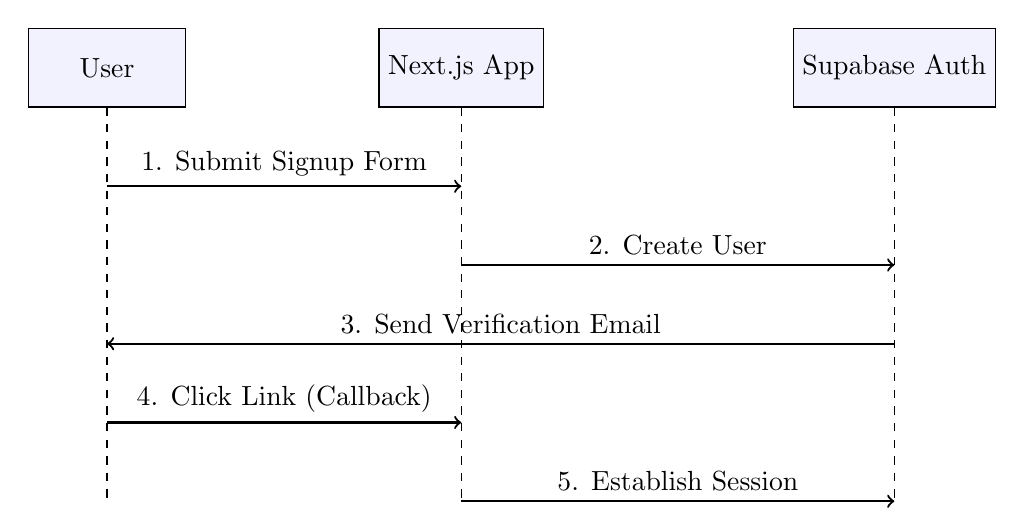
\begin{tikzpicture}[
        node distance=2.5cm,
        auto,
        box/.style={rectangle, draw, minimum width=2cm, minimum height=1cm, align=center, fill=blue!5},
        arrow/.style={->, thick}
    ]
    
    \node[box] (user) {User};
    \node[box, right of=user, xshift=2cm] (next) {Next.js App};
    \node[box, right of=next, xshift=3cm] (supa) {Supabase Auth};
    
    \draw[dashed] (user.south) -- +(0,-5cm);
    \draw[dashed] (next.south) -- +(0,-5cm);
    \draw[dashed] (supa.south) -- +(0,-5cm);
    
    \draw[arrow] ([yshift=-1cm]user.south) -- node[above] {1. Submit Signup Form} ([yshift=-1cm]next.south);
    \draw[arrow] ([yshift=-2cm]next.south) -- node[above] {2. Create User} ([yshift=-2cm]supa.south);
    \draw[arrow] ([yshift=-3cm]supa.south) -- node[above] {3. Send Verification Email} ([yshift=-3cm]user.south);
    \draw[arrow] ([yshift=-4cm]user.south) -- node[above] {4. Click Link (Callback)} ([yshift=-4cm]next.south);
    \draw[arrow] ([yshift=-5cm]next.south) -- node[above] {5. Establish Session} ([yshift=-5cm]supa.south);
    
    \end{tikzpicture}
    \caption{Authentication Sequence Diagram}
    \label{fig:auth_flow}
\end{figure}

\section{Key Portal Features}

\subsection{E-Commerce and Product Management}
The "Summit Gear" store allows users to browse climbing equipment and the tracker devices.
The system implements a standard e-commerce flow: Product Browsing $\rightarrow$ Cart $\rightarrow$ Checkout. Administrators can manage product listings, update stock levels, and process incoming orders via a protected admin dashboard.

\begin{figure}[htbp]
    \centering
    
\includegraphics[width=0.9\textwidth]{portal_store.png}
    \caption{Summit Gear E-Commerce Interface}
    \label{fig:portal_store}
\end{figure}

\subsection{Device Registration Workflow}
When a user purchases a Climber Health Tracker, they must register the device on the portal using a unique serial number. 
This workflow links the physical device's MAC address and LoRa Node ID to the user's account in the PostgreSQL database. Row-Level Security (RLS) in Supabase ensures that users can only view and manage devices registered to their own account.

\subsection{Firmware Downloads}
The portal provides a secure section for registered users to download the latest OTA (Over-The-Air) firmware binaries. The Next.js backend verifies the user's session and device ownership before granting access to the firmware files stored in Supabase Storage.
